\documentclass[tikz,border=6pt]{standalone}
\usepackage{amsmath,amssymb,bm}
\usepackage{tikz}
\usetikzlibrary{arrows.meta,calc,positioning,fit,backgrounds,decorations.pathreplacing,shapes.geometric,quotes}
\definecolor{okBlue}{HTML}{4472C4}
\definecolor{okRed}{HTML}{C0504D}
\definecolor{okGreen}{HTML}{55A868}
\definecolor{okOrange}{HTML}{D98E04}
\definecolor{okPurple}{HTML}{7E57C2}
\definecolor{okGray}{HTML}{666666}
\definecolor{softBlue}{HTML}{EAF1FB}
\definecolor{softRed}{HTML}{F9ECEB}
\definecolor{softGreen}{HTML}{EDF7F0}
\tikzset{
  >={Latex[length=2.2mm,width=2.0mm]},
  every node/.style={font=\small},
  mathbox/.style={draw=black!55, rounded corners=2pt, very thick, fill=black!2, inner sep=5pt, align=center},
  chip/.style={draw=black!45, rounded corners=1.6pt, fill=black!1, inner sep=2pt, align=center},
  panel/.style={draw=black!55, rounded corners=2pt, line width=0.8pt},
  lightpanel/.style={draw=black!25, rounded corners=2pt, line width=0.5pt},
  flow/.style={-{Latex[length=2.3mm]}, line width=1.0pt, draw=black!70},
  thinflow/.style={-{Latex[length=1.9mm]}, line width=0.8pt, draw=black!55},
  faintcol/.style={draw=black!18, line width=0.6pt},
  reglabel/.style={font=\normalsize},
  srcA/.style={circle, draw=okBlue!70!black, fill=okBlue!15, minimum size=5.2pt, inner sep=0pt},
  srcB/.style={circle, draw=okRed!70!black, fill=okRed!15, minimum size=5.2pt, inner sep=0pt},
  tgtA/.style={circle, draw=okBlue!70!black, fill=okBlue!15, minimum size=5.2pt, inner sep=0pt},
  tgtB/.style={circle, draw=okRed!70!black, fill=okRed!15, minimum size=5.2pt, inner sep=0pt},
  crossdot/.style={diamond, draw=okOrange!80!black, fill=okOrange!85, minimum size=6pt, inner sep=0pt},
  kedge/.style={draw=okBlue!60!black, line width=0.9pt, opacity=0.50},
  triangleedge/.style={draw=okRed!75!black, line width=1.1pt, opacity=0.55},
  matching/.style={draw=okGreen!70!black, line width=1.8pt},
  absent/.style={draw=black!15, dashed, line width=0.55pt},
  qdata/.style={circle, fill=okGreen!75!black, draw=okGreen!55!black, minimum size=4.2pt, inner sep=0pt},
  qx/.style={rectangle, draw=okPurple!85!black, fill=white, minimum size=5.3pt, inner sep=0pt, line width=0.7pt},
  qz/.style={diamond, draw=okOrange!85!black, fill=white, minimum size=5.3pt, inner sep=0pt, line width=0.7pt},
  routeA/.style={draw=okBlue!85!black, line width=1.15pt, line cap=round, line join=round},
  routeB/.style={draw=okRed!85!black, line width=1.15pt, line cap=round, line join=round},
  access/.style={draw=black!40, densely dotted, line width=0.55pt},
  layA/.style={draw=okBlue!55!black, fill=okBlue!10, line width=0.7pt},
  layB/.style={draw=okRed!55!black, fill=okRed!10, line width=0.7pt},
  layBase/.style={draw=black!35, fill=black!5, line width=0.7pt},
  titleline/.style={font=\normalsize\bfseries},
  paneltag/.style={font=\bfseries\normalsize},
}

\begin{document}
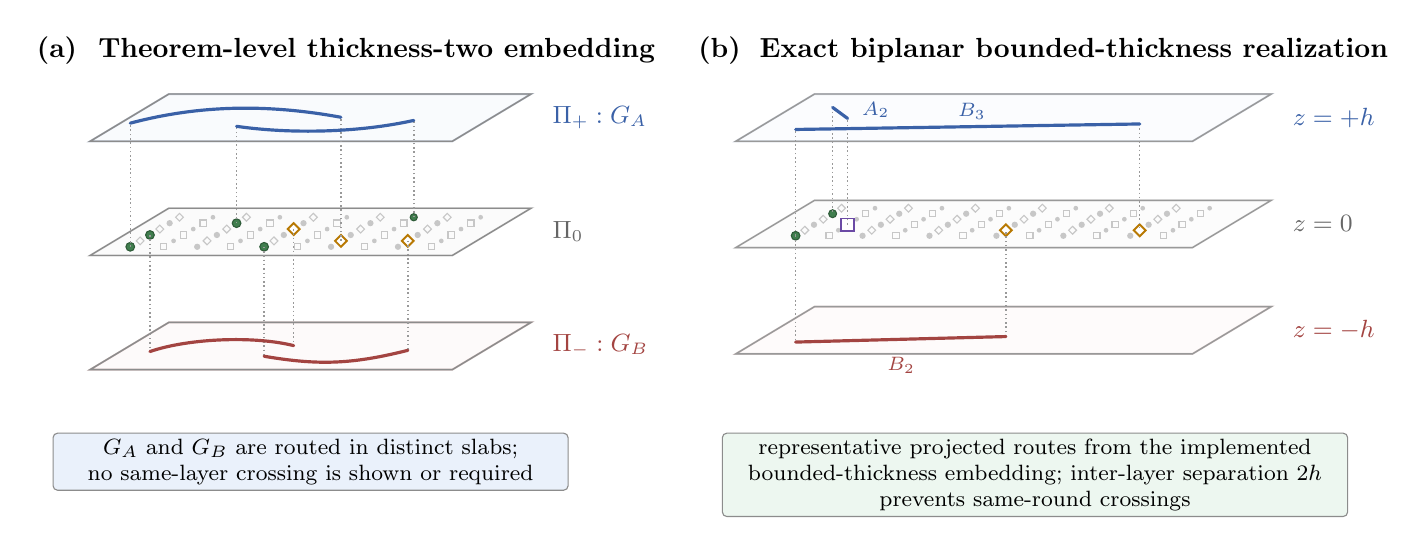
\begin{tikzpicture}[x=1cm,y=1cm]

% ====================================================================
% PANEL (a): Theorem-level thickness-two embedding
% ====================================================================
\node[paneltag, anchor=west] at (0.00,5.10) {\textbf{(a)}};
\node[titleline, anchor=west] at (0.78,5.10)
  {Theorem-level thickness-two embedding};

% Three oblique parallelogram slabs
\coordinate (aUp1) at (0.80,3.95);
\coordinate (aUp2) at (5.40,3.95);
\coordinate (aUp3) at (6.40,4.55);
\coordinate (aUp4) at (1.80,4.55);
\coordinate (aMid1) at (0.80,2.50);
\coordinate (aMid2) at (5.40,2.50);
\coordinate (aMid3) at (6.40,3.10);
\coordinate (aMid4) at (1.80,3.10);
\coordinate (aLo1) at (0.80,1.05);
\coordinate (aLo2) at (5.40,1.05);
\coordinate (aLo3) at (6.40,1.65);
\coordinate (aLo4) at (1.80,1.65);

\fill[layA, opacity=0.30] (aUp1)--(aUp2)--(aUp3)--(aUp4)--cycle;
\fill[layBase, opacity=0.32] (aMid1)--(aMid2)--(aMid3)--(aMid4)--cycle;
\fill[layB, opacity=0.30] (aLo1)--(aLo2)--(aLo3)--(aLo4)--cycle;
\draw[black!45, line width=0.5pt] (aUp1)--(aUp2)--(aUp3)--(aUp4)--cycle;
\draw[black!45, line width=0.5pt] (aMid1)--(aMid2)--(aMid3)--(aMid4)--cycle;
\draw[black!45, line width=0.5pt] (aLo1)--(aLo2)--(aLo3)--(aLo4)--cycle;

% Slab labels
\node[anchor=west, text=okBlue!85!black, font=\small]
  at (6.55,4.25) {$\Pi_+ : G_A$};
\node[anchor=west, text=black!60, font=\small]
  at (6.55,2.80) {$\Pi_0$};
\node[anchor=west, text=okRed!85!black, font=\small]
  at (6.55,1.35) {$\Pi_- : G_B$};

% ── Toric base patch on Π₀ ──
% Π₀ slab: (0.80,2.50)–(5.40,2.50)–(6.40,3.10)–(1.80,3.10), width 4.60, depth 0.60.
% Slab shear ratio: Δx/Δy = 1.00/0.60 = 5/3.
% 5×3 unit-cell grid; oblique basis matched to slab shear.
\def\ox{1.31}   \def\oy{2.61}   % origin (centered within slab)
\def\sx{0.85}   \def\sy{0.00}   % column step (along front edge)
\def\rx{0.25}   \def\ry{0.15}   % row step (oblique depth, shear = 5/3)
% Sub-cell offsets: exact half-cell positions in the 2×2 toric register layout.
%   q(L) at (2a,2b)     →  (0, 0)             within the cell
%   q(X) at (2a+1,2b)   →  (sx/2, 0)   = (0.425, 0.000)
%   q(Z) at (2a,2b+1)   →  (rx/2, ry/2) = (0.125, 0.075)
%   q(R) at (2a+1,2b+1) →  (sx/2+rx/2, ry/2) = (0.550, 0.075)
\def\dXx{0.425} \def\dXy{0.000}
\def\dZx{0.125} \def\dZy{0.075}
\def\dRx{0.550} \def\dRy{0.075}

% Inactive qubits — show register types at every grid point
\foreach \col in {0,1,2,3,4} {
  \foreach \row in {0,1,2} {
    \pgfmathsetmacro{\bx}{\ox + \col*\sx + \row*\rx}
    \pgfmathsetmacro{\by}{\oy + \col*\sy + \row*\ry}
    % L site (green circle, grayed)
    \fill[black!22] (\bx,\by) circle (0.040);
    % X site (purple square, grayed) — centered at half-column
    \draw[black!22, line width=0.4pt]
      ({\bx+\dXx-0.04},{\by+\dXy-0.04}) rectangle ++(0.08,0.08);
    % Z site (orange diamond, grayed) — at half-row
    \node[diamond, draw=black!22, fill=none, minimum size=3pt, inner sep=0pt,
          line width=0.4pt] at ({\bx+\dZx},{\by+\dZy}) {};
    % R site (green circle, grayed, smaller) — at half-col + half-row
    \fill[black!22] ({\bx+\dRx},{\by+\dRy}) circle (0.030);
  }
}

% ── Active endpoints (highlighted, non-crossing route plan) ──
% Blue route 1: L(0,0) → Z(3,0)   — front row, left to right
\pgfmathsetmacro{\bAsx}{\ox + 0*\sx + 0*\rx}
\pgfmathsetmacro{\bAsy}{\oy + 0*\sy + 0*\ry}
\pgfmathsetmacro{\bAtx}{\ox + 3*\sx + 0*\rx + \dZx}
\pgfmathsetmacro{\bAty}{\oy + 3*\sy + 0*\ry + \dZy}
\fill[qdata] (\bAsx,\bAsy) circle (0.055);
\node[qz, scale=0.85] at (\bAtx,\bAty) {};

% Blue route 2: L(1,2) → R(3,2)   — back row
\pgfmathsetmacro{\bBsx}{\ox + 1*\sx + 2*\rx}
\pgfmathsetmacro{\bBsy}{\oy + 1*\sy + 2*\ry}
\pgfmathsetmacro{\bBtx}{\ox + 3*\sx + 2*\rx + \dRx}
\pgfmathsetmacro{\bBty}{\oy + 3*\sy + 2*\ry + \dRy}
\fill[qdata] (\bBsx,\bBsy) circle (0.055);
\fill[qdata] (\bBtx,\bBty) circle (0.045);

% Red route 1: L(0,1) → Z(2,1)    — middle row, left to right
\pgfmathsetmacro{\rAsx}{\ox + 0*\sx + 1*\rx}
\pgfmathsetmacro{\rAsy}{\oy + 0*\sy + 1*\ry}
\pgfmathsetmacro{\rAtx}{\ox + 2*\sx + 1*\rx + \dZx}
\pgfmathsetmacro{\rAty}{\oy + 2*\sy + 1*\ry + \dZy}
\fill[qdata] (\rAsx,\rAsy) circle (0.055);
\node[qz, scale=0.85] at (\rAtx,\rAty) {};

% Red route 2: L(2,0) → Z(4,0)    — front row, right portion
\pgfmathsetmacro{\rBsx}{\ox + 2*\sx + 0*\rx}
\pgfmathsetmacro{\rBsy}{\oy + 2*\sy + 0*\ry}
\pgfmathsetmacro{\rBtx}{\ox + 4*\sx + 0*\rx + \dZx}
\pgfmathsetmacro{\rBty}{\oy + 4*\sy + 0*\ry + \dZy}
\fill[qdata] (\rBsx,\rBsy) circle (0.055);
\node[qz, scale=0.85] at (\rBtx,\rBty) {};

% ── Access lines ──
% Target endpoints raised by dZy=0.075 or dRy=0.075 to match base-plane depth offset.
\draw[access] (\bAsx,\bAsy)--(\bAsx,4.18);
\draw[access] (\bAtx,\bAty)--(\bAtx,4.255);
\draw[access] (\bBsx,\bBsy)--(\bBsx,4.14);
\draw[access] (\bBtx,\bBty)--(\bBtx,4.215);
\draw[access] (\rAsx,\rAsy)--(\rAsx,1.28);
\draw[access] (\rAtx,\rAty)--(\rAtx,1.355);
\draw[access] (\rBsx,\rBsy)--(\rBsx,1.22);
\draw[access] (\rBtx,\rBty)--(\rBtx,1.295);

% ── Blue curves in Π+ (non-intersecting, slopes match base-plane Δy) ──
\draw[routeA] (\bAsx,4.18)
  .. controls ({\bAsx+0.9},4.42) and ({\bAtx-0.9},4.42) .. (\bAtx,4.255);
\draw[routeA] (\bBsx,4.14)
  .. controls ({\bBsx+0.7},4.04) and ({\bBtx-0.7},4.06) .. (\bBtx,4.215);

% ── Red curves in Π- (non-crossing, slopes match base-plane Δy) ──
\draw[routeB] (\rAsx,1.28)
  .. controls ({\rAsx+0.5},1.45) and ({\rAtx-0.5},1.48) .. (\rAtx,1.355);
\draw[routeB] (\rBsx,1.22)
  .. controls ({\rBsx+0.7},1.10) and ({\rBtx-0.7},1.12) .. (\rBtx,1.295);

% Chip below panel (a)
\node[chip, fill=softBlue, anchor=north, align=center,
      text width=6.4cm, font=\footnotesize]
  at (3.60,0.25)
  {$G_A$ and $G_B$ are routed in distinct slabs;\\
   no same-layer crossing is shown or required};

% ====================================================================
% PANEL (b): Exact biplanar bounded-thickness realization
% ====================================================================
\node[paneltag, anchor=west] at (8.40,5.10) {\textbf{(b)}};
\node[titleline, anchor=west] at (9.18,5.10)
  {Exact biplanar bounded-thickness realization};

% Slab shear Δ=(1.00,0.60), matching panel (a) perspective exactly.
% Single slabs per layer — the inter-layer separation 2h is the
% theorem-facing quantity; intra-layer εᵢ offsets are infinitesimal
% computational regularizations, not visible at this scale.

% ── Π+ routing slab ──
\fill[layA, opacity=0.22]
  (9.00,3.95)--(14.80,3.95)--(15.80,4.55)--(10.00,4.55)--cycle;
\draw[black!40, line width=0.5pt]
  (9.00,3.95)--(14.80,3.95)--(15.80,4.55)--(10.00,4.55)--cycle;

% ── Π₀ base slab ──
\fill[layBase, opacity=0.26]
  (9.00,2.60)--(14.80,2.60)--(15.80,3.20)--(10.00,3.20)--cycle;
\draw[black!40, line width=0.5pt]
  (9.00,2.60)--(14.80,2.60)--(15.80,3.20)--(10.00,3.20)--cycle;

% ── Π- routing slab ──
\fill[layB, opacity=0.22]
  (9.00,1.25)--(14.80,1.25)--(15.80,1.85)--(10.00,1.85)--cycle;
\draw[black!40, line width=0.5pt]
  (9.00,1.25)--(14.80,1.25)--(15.80,1.85)--(10.00,1.85)--cycle;

% z-level labels
\node[anchor=west, text=okBlue!85!black, font=\small]
  at (15.95,4.25) {$z=+h$};
\node[anchor=west, text=black!60, font=\small]
  at (15.95,2.90) {$z=0$};
\node[anchor=west, text=okRed!85!black, font=\small]
  at (15.95,1.55) {$z=-h$};

% ── Toric base patch on Π₀ (proper grid, matching panel (a)) ──
% Π₀(b) slab: (9.00,2.60)–(14.80,2.60)–(15.80,3.20)–(10.00,3.20)
% Width 5.80, depth 0.60, shear 1.00/0.60 = 5/3 (matches panel (a)).
% 6 columns × 3 rows; oblique basis matched to slab shear.
\def\ox{9.76}   \def\oy{2.75}
\def\sx{0.85}   \def\sy{0.00}
\def\rx{0.233}  \def\ry{0.14}
\def\dXx{0.425} \def\dXy{0.000}
\def\dZx{0.117} \def\dZy{0.070}
\def\dRx{0.542} \def\dRy{0.070}

% Inactive qubits (6 columns × 3 rows)
\foreach \col in {0,1,2,3,4,5} {
  \foreach \row in {0,1,2} {
    \pgfmathsetmacro{\bx}{\ox + \col*\sx + \row*\rx}
    \pgfmathsetmacro{\by}{\oy + \col*\sy + \row*\ry}
    \fill[black!22] (\bx,\by) circle (0.040);
    \draw[black!22, line width=0.4pt]
      ({\bx+\dXx-0.04},{\by+\dXy-0.04}) rectangle ++(0.08,0.08);
    \node[diamond, draw=black!22, fill=none, minimum size=3pt, inner sep=0pt,
          line width=0.4pt] at ({\bx+\dZx},{\by+\dZy}) {};
    \fill[black!22] ({\bx+\dRx},{\by+\dRy}) circle (0.030);
  }
}

% Active route endpoints (highlighted on top of the gray grid)
\fill[qdata] (9.76,2.75) circle (0.055);          % B₃ & B₂ source: L(0,0)
\node[qx, scale=0.85] at (10.42,2.89) {};          % A₂ source: X(0,1)
\fill[qdata] (10.23,3.03) circle (0.050);          % A₂ target: L(0,2)
\node[qz, scale=0.85] at (12.43,2.82) {};          % B₂ target: Z(3,0)
\node[qz, scale=0.85] at (14.13,2.82) {};          % B₃ target: Z(5,0)

% ── Access lines and traverses (implementation routes) ──
% Access lines (dotted, matching panel (a) convention) show layer
% entry/exit.  Traverses (solid) show the in-plane routing.
% Traverse slopes match base-plane (Δx,Δy) between source and
% target, preserving the oblique perspective.
% A₂ connects X(0,1)→L(0,2) (rows 1→2, deeper in slab);
% B₃ connects L(0,0)→Z(5,0) (row 0, front of slab).
% Natural depth separation avoids projection crossing.
% Draw order: A₂ first (deeper), then B₃ (front, on top).

% A₂ access lines — X(0,1) at row 1 → L(0,2) at row 2
\draw[access] (10.42,2.89) -- (10.42,4.24);    % X(0,1) lift to Π+
\draw[access] (10.23,4.38) -- (10.23,3.03);    % descend to L(0,2)
% A₂ traverse (base Δ=(−0.19,+0.14), naturally deeper in slab)
\draw[routeA] (10.42,4.24) -- (10.23,4.38);
\node[text=okBlue!85!black, font=\scriptsize, anchor=west]
  at (10.48,4.35) {$A_2$};

% B₃ access lines — L(0,0) → Z(5,0), both row 0 (front of slab)
\draw[access] (9.76,2.75) -- (9.76,4.10);      % L(0,0) lift to Π+
\draw[access] (14.13,4.17) -- (14.13,2.82);    % descend to Z(5,0)
% B₃ traverse (base Δ=(+4.37,+0.07))
\draw[routeA] (9.76,4.10) -- (14.13,4.17);
\node[text=okBlue!85!black, font=\scriptsize, anchor=south]
  at (12.00,4.10) {$B_3$};

% B₂ access lines — L(0,0) → Z(3,0), both row 0
\draw[access] (9.76,2.75) -- (9.76,1.40);      % L(0,0) descend to Π-
\draw[access] (12.43,1.47) -- (12.43,2.82);    % ascend to Z(3,0)
% B₂ traverse (base Δ=(+2.67,+0.07))
\draw[routeB] (9.76,1.40) -- (12.43,1.47);
\node[text=okRed!85!black, font=\scriptsize, anchor=north]
  at (11.10,1.33) {$B_2$};

% Chip below panel (b)
\node[chip, fill=softGreen, anchor=north, align=center,
      text width=7.8cm, font=\footnotesize]
  at (12.80,0.25)
  {representative projected routes from the implemented\\
   bounded-thickness embedding; inter-layer separation $2h$\\
   prevents same-round crossings};

\end{tikzpicture}
\end{document}
